% Classe do documento e parâmetros gerais.
\documentclass[a4paper,openright,twoside,11pt]{report}

%
% Times New Roman font.
%
\usefont{T1}{ptm}{m}{n}
\selectfont

% Packages a utilizar e respetivos parâmetros.
\usepackage[utf8]{inputenc}
\usepackage[portuguese]{babel}
\usepackage{graphicx}
\usepackage{url}
\usepackage[Algoritmo]{algorithm}
\usepackage{algorithmicx}
\usepackage{algpseudocode}
\usepackage{indentfirst}
\usepackage[utf8]{inputenc}
\usepackage[toc, acronym]{glossaries}
\usepackage[final]{pdfpages}
\usepackage{pdflscape}
\usepackage[normalem]{ulem} % Sublinhar a Tracejado
\usepackage{tabularx}
\usepackage{multirow}
\usepackage{array}
\usepackage[section]{placeins}
\usepackage{amssymb}% http://ctan.org/pkg/amssymb
\usepackage{pifont}% http://ctan.org/pkg/pifont


\addto{\captionsportuguese}{\renewcommand{\bibname}{Refer\^{e}ncias}}
\addto{\captionsportuguese}{\renewcommand{\contentsname}{\'Indice}}
\addto{\captionsportuguese}{\renewcommand{\appendixname}{Anexo}}

\renewcommand{\algorithmicrequire}{\textbf{Dados: }}
\renewcommand{\algorithmicensure}{\textbf{Resultado: }}

\newcommand{\cmark}{\ding{51}}%
\newcommand{\xmark}{\ding{55}}%

\newcolumntype{L}[1]{>{\raggedright\let\newline\\\arraybackslash\hspace{0pt}}m{#1}}
\newcolumntype{C}[1]{>{\centering\let\newline\\\arraybackslash\hspace{0pt}}m{#1}}
\newcolumntype{R}[1]{>{\raggedleft\let\newline\\\arraybackslash\hspace{0pt}}m{#1}}

% Definições das dimensões das páginas
\setlength{\textheight}{24.00cm}
\setlength{\textwidth}{15.50cm}
\setlength{\topmargin}{0.35cm}
\setlength{\headheight}{0cm}
\setlength{\headsep}{0cm}
\setlength{\oddsidemargin}{0.25cm}
\setlength{\evensidemargin}{0.25cm}

%
% Times New Roman font.
%
\usefont{T1}{ptm}{m}{n}
\selectfont

% Glossários
\makeglossaries

% Abreviaturas
\label{abreviaturas}
 
\newacronym{w3c}{W3C}{\textit{World Wide Web Consortium}}
\newacronym{cors}{CORS}{\textit{Cross-Origin Resource Sharing}}
\newacronym{log}{Log}{\textit{Linear observations guide}}
 % Tecnologias
\newacronym{nfc}{NFC}{\textit{Near-Field Communication}}
\newacronym{rfid}{RFID}{\textit{Radio-frequency Identification}}
\newacronym{iot}{IoT}{\textit{Internet of Things}}
\newacronym{ip}{IP}{\textit{Internet Protocol}}
\newacronym{uri}{URI}{\textit{Uniform Resource Identifier}}

% Ferramentas
\newacronym{sgbd}{SGBD}{Sistema de Gestão de Base de Dados}
\newacronym{sgbdr}{SGBDR}{Sistema de Gestão de Base de Dados Relacional}
\newacronym{orm}{ORM}{Object-relational mapping}
\newacronym{jpa}{JPA}{\textit{Java Persistent API}}
\newacronym{jdbc}{JDBC}{\textit{Java Database Connectivity}}
\newacronym{jdbctemplate}{Jdbc \textit{Template}}{\textit{Java Database Connectivity Template}}
\newacronym{apk}{APK}{\textit{Android Package}}
% Camadas
\newacronym{bd}{BD}{Base de Dados}
\newacronym{dal}{DAL}{Camada de Acesso a Dados}
\newacronym{bll}{BLL}{Camada da Lógica de Negócio}


% Formato
\newacronym{json}{JSON}{\textit{JavaScript Object Notation}}
\newacronym{pojo}{POJO}{\textit{Plain Old Java Objects}}
\newacronym{csv}{CSV}{\textit{Comma-separated values}}

% Gestão de Stocks
\newacronym{sku}{SKU}{\textit{Stock Keeping Unit}}

% Modelo Relacional
\newacronym{cp}{CP}{Chave-Primária}
\newacronym{ce}{CE}{Chave-Estrangeira}
\newacronym{occ}{OCC}{Outra Chave-Candidata}

%Propriedades/Caraterísticas
\newacronym{acid}{ACID}{\textit{Atomicity, Consistency, Isolation, Durability}}
\newacronym{mvcc}{MVCC}{\textit{Multiversion Concurrency Control}}
\newacronym{crud}{CRUD}{\textit{Create, Read, Update e Delete}}

%Protocolos
\newacronym{http}{HTTP}{\textit{Hypertext Transfer Protocol}}
\newacronym{https}{HTTPS}{\textit{Hypertext Transfer Protocol Secure}}

%Padrões
\newacronym{mvc}{MVC}{\textit{Model-View-Controller}}
\newacronym{mvp}{MVP}{\textit{Model-View-Presenter}}
\newacronym{mvvm}{MVVM}{\textit{Model-View-ViewModel}}

\newacronym{uml}{UML}{\textit{Unified Modeling Language}}
\newacronym{xml}{XML}{\textit{Extensible Markup Language}}
\newacronym{url}{URL}{\textit{Uniform Resource Locator}}

% \acrlong{ } 
% Displays the phrase which the acronyms stands for. Put the label of the acronym inside the braces. In the example, \acrlong{gcd} prints Greatest Common Divisor.

% \acrshort{ } 
%Prints the acronym whose label is passed as parameter. For instance, \acrshort{gcd} renders as GCD.

%\acrfull{ } 
%Prints both, the acronym and its definition. In the example the output of \acrfull{lcm} is Least Common Multiple (LCM).

% Terminologia
\label{terminologia}

\newglossaryentry{api}
{
	name=API,
	description={Web APIs are Application Programming Interfaces. Interfaces to information and functionality provided by systems, used by other applications.}
}

\newglossaryentry{api-web}
{
	name={API Web},
	description={Web APIs are Application Programming Interfaces. Interfaces to information and functionality provided by systems, used by other applications.}
}

\newglossaryentry{open-source}
{
	name={\textit{open source}},
	description={Modelo de desenvolvimento, no qual o código-fonte é disponibilizado sendo assim possível para qualquer pessoa estudar, alterar e distribuir o software seja com que finalidade for.}
}

%
% Página inicial (capa)
%
\title{
   \vspace{-60mm}
   \begin{minipage}[l]{160mm}
   	\resizebox{90mm}{!}{
\includegraphics{./figures/logo_ISEL_principal_PNG.png}}\\
   \end{minipage}\\
   \vspace{15mm}
   % Título do projeto na forma capitalizada. A primeira letra de cada palavra deve ser maiúscula.
   {\bf Gestão Inteligente de Stocks}
}

% Nome dos autores (um por linha)
\author{
	\begin{tabular}{ll}
		& Ana Santos \\
		& Inês Soares \\
		& Nuno Veloso \\
	\end{tabular}
}


\date{
	\vspace{80mm}
	\begin{tabular}{ll}
		{Orientadores} & Matilde Pato \\
		& Nuno Datia \\
	\end{tabular}\\
	% Deixar o indicador respetivo em função da versão do relatório.
	\vspace{10mm}
	Relatório beta realizado no âmbito de Projeto e Seminário,\\
	do curso de licenciatura em Engenharia Informática e de Computadores\\
	Semestre de Verão 2017/2018\\
	\vspace{20mm}
	Maio de 2018
}

\begin{document}

\pagenumbering{roman}
\thispagestyle{empty}
\maketitle
\raggedbottom

\baselineskip 18pt % line spacing: 12pt for single, 18pt for 1 1/2, and 24pt for double spacing

\newpage
\thispagestyle{empty}
% Fim da contracapa

% Página com identificação completa (número e nome) e assinaturas dos estudante(s) e do(s) orientador(es)
\cleardoublepage\newpage
\setcounter{page}{1}
\begin{center}
{\Large\bf Instituto Superior de Engenharia de Lisboa}\\
{\large Licenciatura em Engenharia Informática e de Computadores}\\
%Projecto e Seminário\\
\vspace{46mm}
{\large \bf  Gestão Inteligente de Stocks}\\
\vspace{16mm}
\begin{tabular}{rl}
  42142 & Ana Rita Ferreira dos Santos\\
  42162 & Inês Lima Amil Soares\\
  42181 & Nuno Manuel Olival Veloso\\
\end{tabular}\\
\vspace{8mm}
\noindent\rule{12cm}{0.6pt}\\
\vspace{8mm}
\noindent\rule{12cm}{0.6pt}\\
\vspace{8mm}
\noindent\rule{12cm}{0.6pt}\\
\vspace{10mm}
\begin{tabular}{rl}
  Orientadores: & Nuno Miguel Soares Datia\\   
                & Matilde Pós-de-Mina Pato\\
\end{tabular}\\
\vspace{8mm}
\noindent\rule{12cm}{0.6pt}\\
\vspace{8mm}
\noindent\rule{12cm}{0.6pt}\\
\vspace{15mm}
Relatório beta realizado no âmbito de Projeto e Seminário,\\
do curso de licenciatura em Engenharia Informática e de Computadores\\
Semestre de Verão 2017/2018\\
\vspace{20mm}
Maio de 2018\\
\end{center}

% Página de resumo em Português
% Página de resumo em Português
\cleardoublepage\newpage
\chapter*{Resumo} \label{resumo}
A gestão de stocks ajuda a controlar, de forma otimizada, os investimentos em stock de uma casa. Com um sistema de gestão apropriado é possível obter diversos benefícios, tais como, acabar com o esquecimento de produtos no fundo dos locais de armazenamento ou fora da validade.
A gestão de stocks envolve três decisões principais:
\begin{itemize}
	\item decidir quando comprar os produtos,
	\item determinar a quantidade a comprar de cada produto e,
	\item garantir um stock mínimo de segurança para cada produto.
\end{itemize}
Estas decisões assumem uma dinâmica que se repete ao longo do tempo. Pretende-se desenvolver um sistema de gestão automática de stocks, onde a recolha de informação é feita por sensores. O sistema é constituído, para além dos sensores, por uma aplicação móvel e web, e um servidor que implementa um algoritmo de previsão de stocks e que disponibiliza uma \gls{api-web}. Este sistema simplifica não só o controlo de stocks, como também a análise dos padrões de consumo e reposição de uma casa. Assim consegue-se auxiliar os utilizadores a manter o stock adequado às suas necessidades, bem como alerta-los para a proximidade do fim da validade e/ou stock dos produtos.

\vspace{0.2cm}
{\bf Palavras-chave: IoT; Gestão de Stock; Previsão de consumo; Sensorização em casa} 

% Página de resumo em Inglês
% Página de resumo em Inglês
\cleardoublepage\newpage
\chapter*{Abstract} \label{abstract}


{\bf Keywords:} 

% Página de agradecimentos
%% Página de agradecimentos
\cleardoublepage\newpage
\chapter*{Agradecimentos} \label{agradecimentos}
Texto dos agradecimentos. É opcional.\\

% Geração do índice de figuras
\listoffigures
\cleardoublepage

% Geração do índice de tabelas
\listoftables
\cleardoublepage

% Geração do índice de Acrónimos e Abreviaturas
%\printglossary[type=\acronymtype, style=long, toctitle={Acronyms}, title={Acronyms}]
%\glsaddall
%\printglossary[]
%\cleardoublepage

% Geração do índice de conteúdos
\cleardoublepage\newpage
\tableofcontents
\cleardoublepage

% Iniciar a numeração de páginas
\setcounter{page}{1}
\pagenumbering{arabic}

% Capitulo 1
%
% Capítulo 1
%
\chapter{Introdução} \label{cap1}

A gestão de stocks é uma tarefa estruturada e repetitiva, para a qual já existem soluções capazes de fornecer listas de compras. \textit{OutOfMilk}\footnote[1]{https://www.outofmilk.com/} e \textit{Bring}\footnote[2]{https://www.getbring.com/\#!/app} são exemplos dessas soluções no formato de aplicações \textit{mobile}. Contudo carecem de controlo de stocks e conhecimento dos hábitos dos seus utilizadores.  Como tal, por meio de uma aplicação \textit{mobile} e \textit{web} com suporte inteligente de um algoritmo de previsão de stocks pretende-se solucionar este problema.

Tendo por base a automatização da recolha de dados recorrendo a sensores, simplifica-se, não só, o controlo de stocks, como também, a análise dos padrões de consumo e reposição numa casa.
Desta forma, auxilia-se os utilizadores a manter o stock adequado às suas necessidades, bem como alertá-los para a proximidade do fim da validade e/ou stock dos produtos. 

Assim, este trabalho vai no sentido de responder a questões como: ``De que forma podemos evitar transtornos causados na altura de reabastecer a nossa despensa? Ou como proceder ao controlo de stocks de alimentos e outros produtos? E como impedir artigos fora de prazo?". Se se entender que uma casa funciona como uma empresa e existem quantidades mínimas recomendadas, é possível gerar uma nota de encomenda com os produtos em falta ou prestes a terminar para o utilizador poder consultar e exercer a compra.

%
% Secção 1.1
%
\section{Contexto} \label{sec11}

Uma boa gestão de stocks de mercadorias é de extrema importância porque tem reflexos imediatos nos resultados de uma empresa, o que permite manter os clientes satisfeitos não só a nível da quantidade como da qualidade. Para manter o stock ideal não basta bom senso e intuição, é necessário conhecer o fluxo de vendas, utilizar ferramentas adequadas de gestão de informação sobre movimentos e eventuais constrangimentos no fornecimento. Extrapolando para a empresa ``casa", o processo é apenas um problema de escala. Organizar a despensa como se de uma empresa se tratasse possibilita uma melhor logística de custos e tempo. Ao elaborar uma lista de stock, onde se vai anotando os produtos que se tem, o que está a acabar e o que se tem de comprar, passa por uma solução indispensável. Que por vezes se torna numa tarefa que ``não é para todos".

Perante este problema, pretende-se desenvolver um sistema, utilizando uma solução digital, aplicação \textit{mobile} e de \textit{web}, que tem como objetivo ajudar os portugueses nesta repetitiva tarefa que é adotar e manter, ao longo do tempo, a sua despensa sem faltas.
Através desta solução, o individuo terá sempre presente informação útil e prática, com possibilidade de utilizar um formato de lembretes e de registar as tendências para uma futura investigação no que diz respeito aos hábitos de consumo.

Destaca-se ainda o facto de, no contexto atual, existir um aumento na facilidade de acesso às novas tecnologias, nomeadamente à \textit{internet}. Em plena era da informação a proliferação dos meios de comunicação e da própria \textit{internet} permitiu que os utilizadores se liguem à rede 24 horas, por dia, através de telemóveis, portáteis, \textit{tablets} e outros. A cada dia que passa assiste-se a uma mudança do comportamento do consumidor nesta área, graças à utilização dos dispositivos móveis dos ``8 aos 80" anos. Conforme os dados divulgados em Dezembro de 2016 pelo Gabinete de Estatísticas da União Europeia (Eurostat) \cite{eurostat:internetAccess2016}.

%
% Secção 1.2
%
\section{Metas e Objetivos} \label{sec12}
Face ao exposto, a existência de um sistema de gestão de stocks na agenda de tarefas de uma organização doméstica poderá ser uma mais valia. Para concretizar esse sistema foi necessário cumprir com objetivos mais específicos que respondessem à seguinte questão: 

``Quais as características e funcionalidades que deverá ter o sistema que sejam úteis para os utilizadores e se diferencia das restantes?"

Deste modo, definiram-se os seguintes objetivos:
\begin{itemize} \itemsep 0pt
	\item Implementar uma interface com o utilizador para dispositivos móveis;
	\item Implementar uma interface com o utilizador para dispositivos \textit{desktop};
	\item Implementar a componente servidora de um sistema de gestão de stocks;
	\item Implementar um algoritmo de previsão de stocks.
\end{itemize}

%
% Secção 1.3
%
\section{Abordagem do Projeto} \label{sec13}

Este trabalho divide-se em duas partes principais. A primeira com o enquadramento teórico, em que se fez uma revisão da literatura focando os principais temas associados ao projeto, nomeadamente, gestão de stocks, a utilização das novas tecnologias. Reviu-se também estratégias de usabilidade e promoção de literatura na construção das aplicações móveis bem como a regulamentação existente e possibilidade de certificação.
Ainda nesta parte, efetuou-se investigação exploratória de suporte à elaboração do projeto, assim como análise e discussão dos resultados obtidos.

Na segunda parte encontra-se todo o trabalho desenvolvido para o projeto. Inicialmente definiram-se os requisitos fundamentais ao sistema de gestão de stocks a desenvolver. Aqui, foi também importante comparar as funcionalidades que se pretendiam implementar com as de outros sistemas já existentes, de forma a garantir elementos inovadores na solução. Posteriormente, definiu-se a arquitetura do sistema tal como todas as partes envolvidas. Foi ainda necessário estabelecer o modo como o utilizador iria interagir com o sistema, através do desenho das interfaces gráficas.

%
% Secção 1.4
%
\section{Estrutura do Relatório} \label{sec14}
Este relatório está organizado em 4 capítulos.

O capítulo 2 introduz o sistema de gestão de stocks desenvolvido, como também, formaliza o problema indicando os requisitos e as entidades para a resolução do mesmo e, ainda, apresenta a solução implementada.

O capítulo 3 aborda as aplicações de interação direta com o utilizador, o desenvolvimento e implementação do algoritmo de previsão de stocks, a \gls{api-web} bem como todas as suas particularidades e a modelagem dada aos dados. Explica de que forma esses dados foram armazenados, sendo ainda apresentadas as justificações das decisões tomadas.

Conclusões e diretrizes relativas a trabalho futuro são disponibilizadas no capítulo 4.

No Anexo A define-se terminologia, quer a básica à gestão de stocks, para melhor compreensão de alguns dos termos utilizados no decorrer do projeto, quer de conceitos de programação.



% Capitulo 2
%
% Capítulo 2
%
\chapter{Formulação do Problema } \label{cap2}

Neste capítulo o problema é descrito de forma detalhada na secção \ref{sec21}, bem como os requisitos funcionais e não funcionais na secção \ref{sec22}. A secção \ref{sec23} apresenta as dificuldades que surgiram no decorrer do projeto. São expostas na secção \ref{sec24} noções da gestão de stocks 


%
% Secção 2.1
%
\section{Descrição do Problema} \label{sec21}
No âmbito do projeto existe a necessidade de criar um sistema de informação que permita gerir os itens em stock de uma dada casa.

Uma casa está associada a um ou mais utilizadores, podendo um utilizador ter várias casas. Cada casa é caracterizada por um identificador único, um nome, atribuído por um utilizador no momento de registo da casa, quantos bebés, crianças, adultos e seniores vivem nessa casa. Cada utilizador é identificado univocamente por um email ou por um nome de utilizador, pelo nome da própria pessoa, idade e uma password. Para cada casa podem existir um ou mais administradores. Um utilizador pode criar as suas listas e as suas receitas. As listas que este cria pode decidir se quer partilhar com os restantes utilizadores da casa a que pertence, nunca podendo partilhar com utilizadores fora da sua casa. Existem listas do sistema que são comuns a todos os utilizadores registados, contudo são particulares a cada casa. As listas partilhadas pelos vários utilizadores dependem dos produtos que cada utilizador tem em casa. As receitas que um utilizador cria podem ser partilhadas com todos os utilizadores registados ou só com determinados utilizadores. Existem ainda um conjunto de receitas que são partilhadas por todos os utilizadores registados.

Cada receita é identificada por um identificador único, um nome, uma preparação, uma dificuldade, um tempo, quantas doses, qual o tipo de cozinha e qual o tipo de prato. Cada receita pode ter vários ingredientes. Para cada receita deve ser possível saber a quantidade dos vários ingredientes que a compõem.
Cada lista é identificada por um identificador único e um nome. Uma lista pode ter vários produtos. Para os produtos presentes numa lista pode ser possível saber a sua marca e a quantidade de um produto na lista. Um produto é identificado pelo seu identificador único, contém um nome, se é comestível ou não, e a validade perecível. Um produto pertence a uma categoria, podendo uma categoria ter vários produtos. Uma categoria é identificada por um identificador único ou um nome. Um produto pode ter vários itens em casa. Uma casa pode ter vários itens presentes na mesma. 

Um item presente numa casa é identificado por um identificador único ou por uma marca, uma variedade e um segmento, é também caracterizado por uma descrição, o local de conservação, a quantidade e as datas de validade. Para cada item deve ser possível saber os seus movimentos, isto é, se entrou ou saiu de um local de armazenamento. Para cada movimento deve ser possível saber o tipo de movimento (entrada ou saída), a data em que ocorreu o movimento e a quantidade de produtos que ocorrem num movimento.
Para cada casa existem vários locais de armazenamento dos itens, por exemplo armários, frigoríficos, etc. Cada local de armazenamento é caraterizado por um identificador único, a temperatura e um nome. Um local de armazenamento pode ter vários itens presentes numa casa e vários movimentos. Para cada local de armazenamento deve ser possível saber a quantidade de cada item.

Para cada casa deve ser possível saber que alergias os seus membros têm e para cada alergia saber o número de membros que têm essa alergia (os membros não precisam necessariamente de estar registados). Deve também ser possível saber os alergénios de um item presente na casa.



%
% Secção 2.2
%
\section{Requisitos Funcionais e Não Funcionais} \label{sec22}

\subsection{Requisitos Funcionais}
\begin{itemize}
	\item Informar o utilizador dos produtos existentes, a sua validade e a sua quantidade;
	\item Alertas sobre os produtos que estão perto da data de validade;
	\item Geração da lista de compras com os produtos em falta;
	\item Possibilidade de especificar os produtos a ter sempre em stock bem como as suas quantidades mínimas;	
	\item Lista de Compras \textit{Offline} (permite rasurar para uso no supermercado);
	\item Listas partilhadas entre utilizadores da mesma casa;
	\item Criação de Listas (As Minhas Listas);
	\item Especificação das alergias dos membros da casa.
\end{itemize}


\subsection{Requisitos Não Funcionais}
\begin{itemize}
	\item Lista de produtos quase a expirar;
	\item Lista de produtos indesejados (Lista Negra);
	\item Lista de contenção em situações de emergência (Lista SOS);
	\item Sugestão de receitas que utilizem os produtos mais perto do fim da validade;
	\item Inserção de receitas (As Minhas Receitas);
	\item Inserir refeições extraordinárias de eventos a realizar num futuro próximo, para acrescentar alimentos não básicos à lista de compras;
	\item Especificação dietas alimentares (Vegetarianos, \textit{Vegans}, etc.) a cada utilizador da casa.
\end{itemize}


%
% Secção 2.3
%
\section{Dificuldades Encontradas} \label{sec23}

Para a realização deste projeto encontrámos dificuldades nos aspetos a seguir referidos.

\subsection{Rótulos em Formato Não Digital}

Nos dias de hoje, os produtos não possuem rótulos digitais. Isto é um problema para a concretização do projeto, na medida em que se torna menos eficiente a recolha dos dados presentes nos produtos. Contudo, assumindo que este dilema é resolvido fora do âmbito do projeto, apenas é preciso definir um formato standard de como os dados devem ser armazenados nas \textit{tags}, que podem ser \acrshort{nfc} ou \acrshort{rfid}. Num cenário ideal, este formato deve ser respeitado por todos os embaladores. Assim, os produtos têm um rótulo, código de barras e uma \textit{tag} \acrshort{nfc} ou \acrshort{rfid}, com a informação necessária. Está fora do âmbito do trabalho implementar o suporte hardware para a leitura das \textit{tags} e qual o sentido do movimento (entrada ou saída). Assume-se que essas informações são disponibilizadas num formato conhecido. 


\subsection{Ausência de Identificador Único nos Itens}

Os itens não dispõem de um identificador unívoco, alguns deles contêm um lote e um número de série. A ausência deste identificador impede a distinção entre itens iguais, o que impossibilita saber se entrou um novo item no local de armazenamento ou se saiu um dos itens presentes. Tal facto torna a gestão dos stocks dependente do dispositivo de hardware para distinguir o tipo de movimento.






% Capitulo 3
%
% Capítulo 3
%
\chapter{Solução Proposta} \label{cap3}

Neste capítulo pretende-se abordar de forma geral a solução implementada para resolver o problema apresentado no capítulo \ref{cap2}.

\begin{figure}[H]
	\centering
	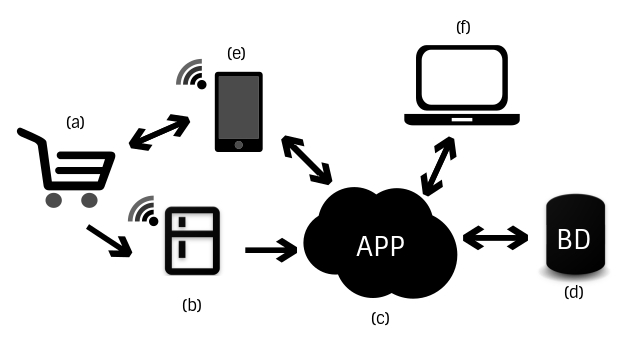
\includegraphics[width=16cm, height=8cm, scale=1]{./figures/architecture.png}
	\caption{Arquitetura Geral do Projeto}
	\label{project-general-architecture}
\end{figure}


A Figura \ref{project-general-architecture} representa o fluxo de dados entre os componentes envolvidos. Com a aquisição dos itens, estes são processados e armazenados nos seus respetivos locais de armazenamento, esta informação é enviada para a API. Estes dados são depois enviados e armazenados de forma persistente na \acrfull{bd}. Quando um dos \textit{endpoint}, \textit{mobile} ou \textit{web}, requisitam esses mesmos dados à API, estes são fornecidos pela \acrshort{bd}, tratados e devolvidos pela API. O fluxo de dados descendente dos \textit{endpoints} para a API acontece aquando o utilizador efetua manipulação de dados. A interação entre o \textit{smartphone} e os itens será posteriormente explicada.

%
% Secção 3.1 Abordagem
%
\section{Abordagem}\label{sec31}

No contexto do projeto assume-se a existência de duas formas de apresentação para os itens em stock: avulsos e embalados. Os primeiros são conservados em sistemas de arrumação identificados com \textit{tags} programáveis por \textit{smartphones}. Os detalhes dos itens são especificados pelo utilizador e carregados para a \textit{tag}. Enquanto que para os produtos embalados, admite-se que os produtores utilizam \textit{tags}, \acrfull{nfc} ou \acrfull{rfid}, para guardar os rótulos de forma digital e em formato standard.

Após a aquisição, os artigos são armazenados em locais que devem dispor de dispositivos de hardware equipados com leitores de \textit{tags}. É recolhida a informação presente na \textit{tag}, identificado o tipo de movimento (entrada ou saída) e enviado para a \gls{api-web}.

\begin{figure}[H]
	\centering
	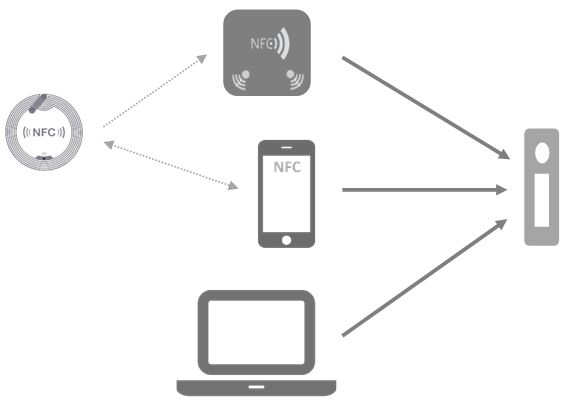
\includegraphics[height=9cm, scale=1]{./figures/project_structures.png}
	\caption{Estrutura do Lado do Cliente Projeto}
	\label{project-structure}
\end{figure}

\begin{figure}[H]
	\centering
	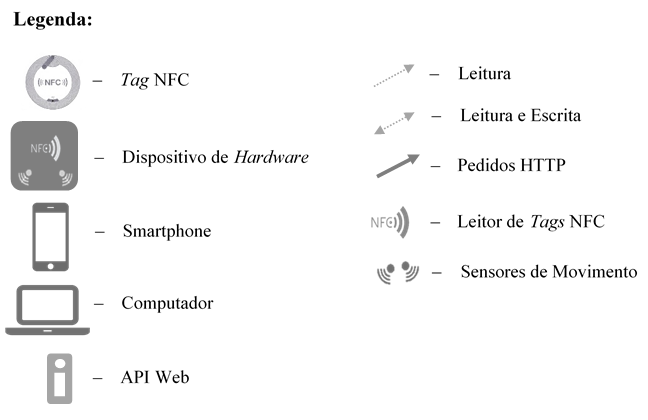
\includegraphics[height=9cm, scale=1]{./figures/project_structures_caption.png}
\end{figure}

Com a Figura \ref{project-structure} pretende-se não só apresentar os principais componentes do projeto, bem como demonstrar de forma breve a relação dos mesmos. É de destacar que uma \textit{tag} pode ser lida por um dispositivo de \textit{hardware} munido de um leitor de \textit{tags}. Assim como um \textit{smartphone}, equipado com tecnologia \acrshort{nfc}, pode escrever na \textit{tag} \acrshort{nfc}, tal é necessário para identificar produtos avulsos presentes num sistema de arrumação. Tanto o dispositivo de \textit{hardware} como as aplicações, móvel e \textit{web}, comunicam com a \gls{api-web}.\\

%
% Secção 3.2 Análise
%
\section{Análise}\label{sec32}

O projeto é composto por 2 blocos principais, que se relacionam. A Figura \ref{project-layers-structure} representa esses blocos. 

\begin{figure}[H]
	\centering
	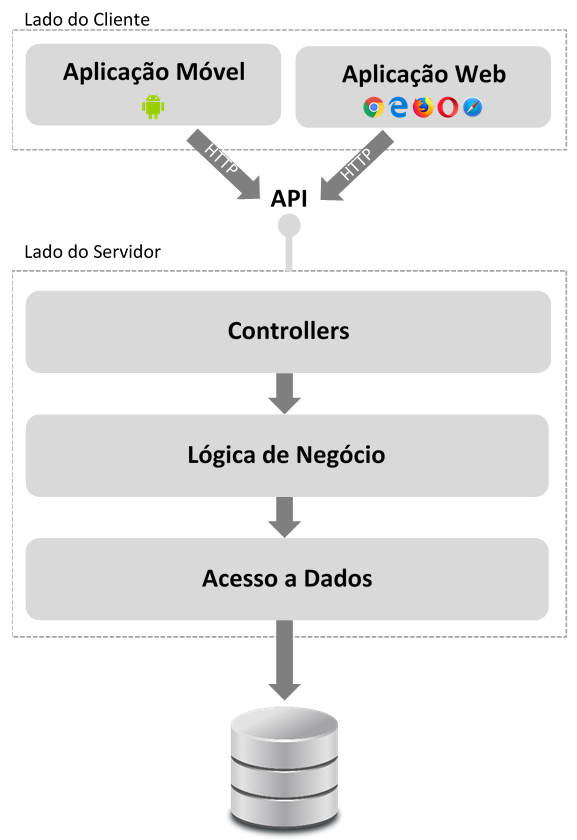
\includegraphics[height=9cm, scale=1]{./figures/project_architecture.png}
	\caption{Estrura por Camadas do Projeto}
	\label{project-layers-structure}
\end{figure}

O lado do servidor incluí quatro camadas e expõe uma \gls{api-web}. A camada da \acrfull{bd} é realizada com o \acrfull{sgbd} \textit{PostgreSQL}. A \acrfull{dal} é responsável pelas leituras e escritas à \acrshort{bd}. Esta camada é produzida com a linguagem de programação \textit{Java}, com a \acrfull{jpa}. A \acrfull{bll} é responsável pela gestão dos dados obtidos da \acrshort{bd} ou dos \textit{controllers}. A implementação desta camada recorreu à mesma ferramenta que foi usada na \acrshort{dal}. Os \textit{controllers} foram desenvolvidos em \textit{Java} com a \textit{framework} da \textit{Spring}, chamada de \textit{Spring Boot}. A \gls{api-web} disponibiliza recursos em diferentes \textit{hypermedia}.

Do lado do cliente existem dois modos de interação, por uma aplicação móvel e outra por uma aplicação web. A aplicação móvel disponível para a plataforma \textit{Android}, desenvolvida em linguagem \textit{Kotlin}. A aplicação web é disponibilizada para a maioria dos browsers, implementada utilizando a linguagem \textit{JavaScript}, com o auxilio da \textit{framework Express}.

%
% Secção 3.3 Dificuldades Encontradas
%
\section{Dificuldades Encontradas} \label{sec33}

Durante a investigação para a resolução deste projeto encontraram-se as seguintes dificuldades.

\subsection{Rótulos em Formato Não Digital}

Nos dias de hoje, os produtos não possuem rótulos digitais. Isto é um problema para a concretização do projeto, na medida em que se torna menos eficiente a recolha dos dados presentes nos produtos. Contudo, assumindo que este problema é resolvido fora do âmbito do projeto, apenas é preciso definir um formato standard de como os dados devem ser armazenados nas \textit{tags}, que podem ser \acrshort{nfc} ou \acrshort{rfid}. Num cenário ideal, este formato deve ser respeitado por todos os embaladores. Assim, os produtos têm um rótulo, código de barras e uma \textit{tag} \acrshort{nfc} ou \acrshort{rfid}, com a informação necessária. Está fora do âmbito do trabalho implementar o suporte hardware para a leitura das \textit{tags} e qual o sentido do movimento (entrada ou saída). Assume-se que essas informações são disponibilizadas num formato conhecido. 


\subsection{Ausência de Identificador Único nos Itens}

Os itens não dispõem de um identificador unívoco. Alguns deles contêm um lote e um número de série. A ausência deste identificador impede a distinção entre itens iguais, o que impossibilita saber se entrou um novo item no local de armazenamento ou se saiu um dos itens presentes. Tal facto torna a gestão dos stocks dependente do dispositivo de hardware para distinguir o tipo de movimento.


% Capitulo 4
%
% Capítulo 4
%
\chapter{Progresso} \label{cap4}

Neste capítulo apresenta-se o progresso do projeto, assim como, o planeamento inicial e de que forma foi cumprido. São  expostas também conclusões face ao desempenho do grupo e trabalho realizado.

\section{Planeamento}\label{sec41}

\section{Web API}\label{sec42}

\section{Algoritmo de Previsão}\label{sec43}

\section{Aplicações Móvel e Web}\label{sec44}





%\section{Base de Dados}\label{sec43}

%\section{Camada de Acesso a Dados}\label{sec44}

%\section{Camada da Lógica de Negócio}\label{sec45}

%\section{Aplicação Móvel}\label{sec47}

%\section{Aplicação Web}\label{sec48}

% Referências
\bibliographystyle{unsrt}
\bibliography{referencias}

% Anexos (opcional)
\appendix

% Anexo 1
%
% Capítulo 1
%
\chapter{Terminologia} \label{a1}

%
% Secção A.1
%
\section{Conceitos Básicos de Gestão de Stocks} \label{seca11}
% Contador de Exemplos
\newcounter{ExampleCounter}

\vspace{0.2cm}
\textbf{Inventário} - Um catálogo detalhado ou uma lista de bens ou propriedades tangíveis, ou os atributos ou qualidades intangíveis. Ler mais em \cite{businessDictionary:invetoryDefinition2018}.

\vspace{0.2cm}
\textbf{\acrfull{sku} (Unidade de Manutenção de Stock, em Português)} - Um código de identificação de um produto e serviço para uma loja ou produto, muitas vezes retratado como um código de barras legível por máquinas que ajuda a rastrear o item para inventários. Ver exemplo \ref{seca11}.1. Ler mais em \cite{investopedia:skuDefinition2018}.

\stepcounter{ExampleCounter}
\noindent\fbox{
	\parbox{\textwidth}{
		\textbf{Exemplo \arabic{ExampleCounter}}\\
		Por exemplo, um armário pode ter  pacotes de leite magro da marca X, 2 pacotes de leite magro da marca Y e 1 pacote de leite meio gordo da marca X. Logo, o armário contém 3 \acrshort{sku}, uma vez que um \acrshort{sku} se distingue pelo tamanho, cor, sabor, marca, etc.
	}
}

\vspace{0.2cm}
\textbf{Stock Item (Item em Stock, em Português)} - Refere-se aos itens que se mantêm em stock físico na loja. O item de stock tem uma quantidade associada. Cada vez que uma venda é feita para aquele item, a sua quantidade será deduzida. 
Artigo aprovado para aquisição, armazenamento e emissão, e geralmente mantido à mão. Ler mais em \cite{businessDictionary:stockItemDefinition2018} e \cite{phostersoft:stockItemDefinition2018}.


\vspace{0.2cm}
\textbf{Product Category (Categoria de Produtos, em Português)} - Taxonomias de classificação que subdividem um Setor ("yet another market construct") nos diferentes tipos de produtos para os quais existe demanda. Quanto mais especializada for uma categoria, mais especializado é o produto. Ler mais em \cite{sphereoi:itemIdentification2018}.

{\footnotesize Nota: Neste projeto apenas se consideram as categorias de maior dimensão, são elas, por exemplo, Laticínios, Bebidas, Frescos, Congelados, entre outras.}

\vspace{0.2cm}
\textbf{Brand (Marca, em Português)} - Um símbolo de identificação, marca, logótipo, nome, palavra e/ou frase que as empresas usam para distinguir os seus produtos dos outros. Ler mais em \cite{investopedia:brandDefinition2018}

\vspace{0.2cm}
\textbf{Segmentation (Segmento, em Português)} - Quando os estrategistas de marca falam sobre segmento,referem-se à segmentação do consumidor/audiência. A maneira antiga de abordar isso era através da demografia (idade, sexo, etnia, faixa de renda, urbano-rural, etc.). Agora a segmentação é VALS (valores, atitudes e estilo de vida). Ler mais em \cite{sphereoi:itemIdentification2018}.

{\footnotesize Nota: Neste projeto o segmento é a quantidade presente numa embalagem, i.e., para um pacote de leite de 1L, o segmento é 1L.}


\vspace{0.2cm}
\textbf{Variety (Variedade, em Português)} - A variedade é confusa porque pode ser difícil de entender onde a especialização da segmentação termina e a especialização em prol da Variedade começa. A variação é sobre a personalização de um produto para se adequar ao caráter do consumidor individual. Ver exemplo \ref{seca11}.2. Ler mais em \cite{sphereoi:itemIdentification2018}.

\vspace{0.5cm}

\stepcounter{ExampleCounter}
\noindent\fbox{
	\parbox{\textwidth}{
		\textbf{Exemplo \arabic{ExampleCounter}}\\	
		Note-se um pacote de leite com as caraterísticas, quantidade líquida igual a 1L, da marca X e do tipo UHT magro. Então, identificar-se-ia da seguinte forma: 
		\begin{itemize}
			\item Categoria: Laticínios
			\item Produto: Leite
			\item Marca: X
			\item Segmento: 1L
			\item Variedade: UHT Magro
		\end{itemize}
	}
}

%
% Secção A.2
%
%\section{Conceitos de ???} \label{seca12}	
	
%\glsaddall
%\printglossary[type=\acronymtype,title=Acrónimos]


% Anexo 2
%\include{anexo2}

\end{document}